\begin{frame}{La caída del FEPC ocultó mayores presiones en otras transferencias}
\centering
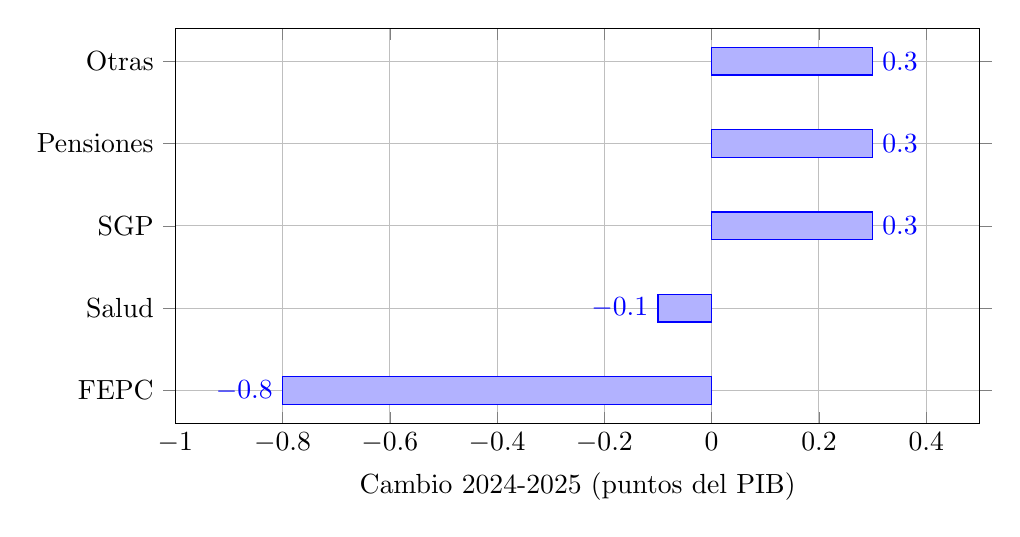
\begin{tikzpicture}
\begin{axis}[
  xbar,
  width=11.8cm,
  height=6.6cm,
  xlabel={Cambio 2024-2025 (puntos del PIB)},
  symbolic y coords={FEPC,Salud,SGP,Pensiones,Otras},
  ytick=data,
  xmin=-1.0,xmax=0.5,
  nodes near coords,
  grid=major
]
\addplot coordinates {(-0.8,FEPC) (-0.1,Salud) (0.3,SGP) (0.3,Pensiones) (0.3,Otras)};
\end{axis}
\end{tikzpicture}
\note{[Sources] MFMP 2026, capítulo 1, gráfico 1.7. Cálculos propios de diferencias.}
\end{frame}